\documentclass[12pt, a4paper, titlepage]{article}
\usepackage{amsthm}
\usepackage{amsmath}
\usepackage{amsfonts}
\usepackage{amssymb}
\setlength{\textheight}{9in}
\setlength{\oddsidemargin}{.125in}
\setlength{\textwidth}{6.25in}
\usepackage{graphicx}
\usepackage{xcolor}
\usepackage{listings}
\lstset{numbers=none,
numberstyle=\tiny,
keywordstyle=\color{blue!70}, 
commentstyle=\color{red!50!green!50!blue!50},
frame=shadowbox,
rulesepcolor=\color{red!20!green!20!blue!20},
basicstyle=\ttfamily\small,
escapeinside=`', %将中文放在`和'之间,可以在lstlisting环境中准确的显示中文
}
\title{\textbf{Financial Data Analysis Group Project}\\
Using ARCH and GARCH Model to Estimate and Forecast CNY Exchange Rate
}
\author{Yufei Li  \\
	32014150004  \\
	\and 
	Yinan Wu \\
	32014150003 \\
	\and
	Ke Zhang\\
	32014150002\\
	\and
	Tianyunzi Chen\\
	32014020199
	}

\date{} 

\begin{document}
\maketitle

\begin{abstract}
The change in the exchange rate reflects the economic situation of a country. The increase or decrease in national income, the development of agriculture, the domestic interest rate, and even the domestic employment are impacted deeply by the change of it. The accuracy of exchange rate forecast has great influence on foreign exchange holders, enterprises' import and export trade, foreign exchange trading of individuals and enterprises, foreign exchange holders and so on. With the continuous development of China's economy, in recent years, China's position in the international community has also been strengthened. At present, the Chinese Yuan(CNY) and the United States Dollar(USD) as the world's most influential two currencies, the exchange rate fluctuations on the global financial and economic development have played a decisive role in the global market.\\

This paper establishes the ARCH model and GARCH model of USD / CNY exchange rate fluctuation, using the daily exchange rate after China has established the exchange rate regime reformation since 2005. Besides, we do a model comparison among different estimated models to try to find a best fitted one. Using AIC and BIC methods of informative criteria and checking the likelihood of the model, we collude that $GARCH(1,1)$ model is the appropriate one to estimate and forecast the USD / CNY exchange rate which can provide some reference for the central bank's control measures and the exchange rate reform policy.\\

\textbf{Key Words: GARCH, ARCH, ARIMA, USD / CNY exchange rate, Comparison, Prediction} 
\end{abstract}
%\begin{keywords}

%\end{keywords}
\tableofcontents 
\newpage

\section{Introduction}
An exchange rate between two currencies is the rate at which one currency will be exchanged for another. It is also regarded as the value of one country's currency in relation to another currency. Exchange rates are determined in the foreign exchange market, which is open to a wide range of different types of buyers and sellers, and where currency trading is continuous. US Dollar(USD) is considered as the most influential currency in the world and many countries have anchored their foreign exchange rate to the dollar. While Chinese Yuan(CNY) shows an increasing power in the international environment. Thus, discussing the relationship between the two currencies is quite meaningful.\\
 
Each country determines the exchange rate regime that will apply to its currency. For example, the currency may be free-floating, pegged (fixed), or a hybrid. The Central Committee and the State Council promulgated the reform of the CNY exchange rate formation mechanism on July 21, 2005. The CNY exchange rate was no longer pegged to a single dollar, and fluctuated according to the market supply and demand. After August 11, 2015, the correlation between the CNY and the dollar index has declined. In 2016, the annual depreciation of CNY is about $6.67\%$, against a basket of currency depreciation rate is $5.13\%$. But the degree of marketization of the CNY in 2016 significantly increased, and gradually drops out of the ``dollar anchor". CNY exchange rate changes as China's international financial relations and even the normal development of economic relations. It is an important link and plays an increasingly important role. Therefore, it has a vital significance to correct analysis and forecast the exchange rate and its volatility for the economic subject of financial policy and investment and financing decision-making undoubtedly. Thus, it is important to choose a satisfactory model to better analyse USD / CNY exchange rate.\\

Many domestic scholars have studied this based on time series measurement method. Which model of ARIMA model, ARCH model or GARCH model is more appropriate for the exchange rate fluctuations is controversial. Zhang(2005) suggested that the exchange rate change was fit into $ARIMA(2,4,5)$ model. Hui(2005) argued that there was a GARCH effect in the time series of USD / CNY, and the $GARCH(1,1)$ model was suitable for USD / CNY modeling. Xu and Li(2007) used the ARMA model to forecast the exchange rate of the euro and yen of a basket of currencies and calculated the future exchange rate of the yuan against the US dollar according to the CNY benchmark exchange rate formula. Liu(2008) selected data of the changes in the daily parity of CNY against the US dollar from Jul.25th, 2005 to Nov.1st, 2007 and stated that the $GARCH(1,1)$ model and the $ARMA(1,1)$ model are all suitable. Zhai(2009) showed that the CNY exchange rate volatility had certain leverage effect and the CNY exchange rate did not have the characteristics of floating exchange rate regime through the TGARCH model empirical study. Luo(2009) analysed the exchange rate volatility model established form the data after the reform of China's exchange rate system. The study shows that there existed ARCH effect in China's foreign exchange market and $GARCH(1,1)$ was suitable for estimating.\\

From previous papers, many studies have been conducted using different techniques of estimation like ARIMA model, ARCH model and GARCH model. But we can also see that some of the papers are using data far from now and have little values of exchange rate after changing the exchange regime. So the past results may be out of date due to the lack of large data set. While right now we gain more data than before, we have the probability to update the model and find a more appropriate one to describe the mean and volatility equations which can provide some reference for further studies.\\

\section{Data Source and Data Description}
\subsection{Data Source}
We collected monthly USD / CNY exchange rate from 1981-01-01 to 2017-06-01, and daily exchange rate data from 2005-07-21 til 2017-06-09 from Federal Reserve System. According to the system, the data are already wiped out the seasonal effect.\\

\subsection{Data Description}
We first use monthly USD / CNY exchange rate data  to plot a trend figure shown as figure \ref{monthly}. According with the news, China used to set fixed exchange rate mechanism before 2015-07-21, the volatility of exchange rate was small. After that date, China started exchange rate regime reforming: announced a move away from the US dollar peg and used a floating exchange rate. Thus in this paper we will mainly focus on analysing exchange rate after the reform.\\ 
\begin{figure}[h!]
\begin{center}
\caption{CNY/ USD Exchange Rate using monthly data}\label{monthly}
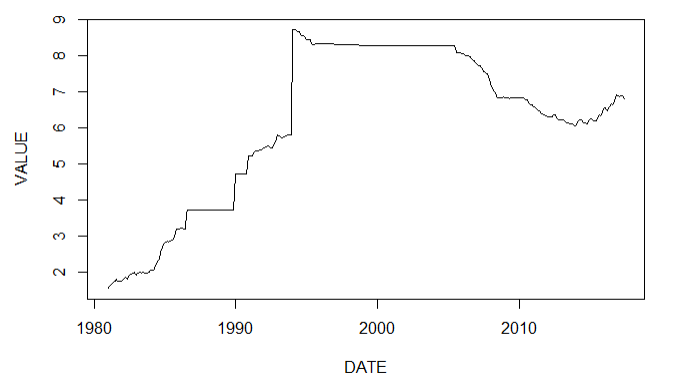
\includegraphics[width=0.6\textwidth]{monthly.png} 
\end{center}
\end{figure}

We collected the daily USD / CNY exchange rate as our data set. The data we found are already wiped out the seasonal effect so we use them directly in examining the model and further doing forecast. We divided the data into two parts one until Jul. 21st, 2016 for examine the model and the data after that date until Jun. 9th, 2017 for checking the evaluation of the models. The trend figure is shown in figure \ref{daily}.\\
\begin{figure}[h!]
\begin{center}
\caption{USD / CNY Exchange Rate using daily data}\label{daily}
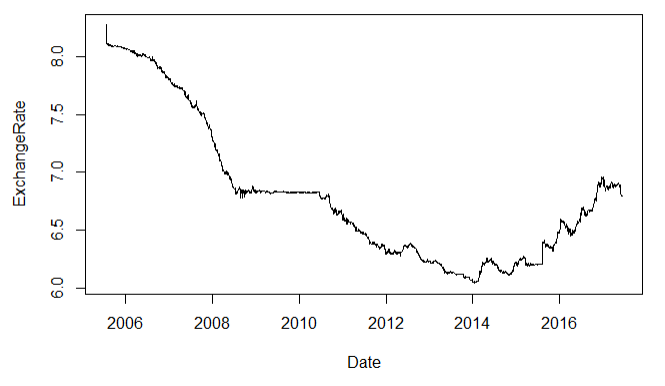
\includegraphics[width=0.6\textwidth]{daily.png} 
\end{center}
\end{figure}

\section{Model Specification}
There are usually two ways in analysing the exchange rate in time series: ARIMA model and GARCH model since they are the more general form of an ARMA model and an ARCH model. 

\subsection{Autoregressive Integrated Moving Average Model}
An Autoregressive Integrated Moving Average(ARIMA) model is a generalization of an Autoregressive Moving Average(ARMA) model with unit roots. Basically an ARMA model combines the ideas of Autocorrelation(AR) model and Moving Average(MA) model but it models with less number of parameters, achieving parsimony in the model. The general $ARMA(p,q)$ form is like $r_t = \phi_0 + \sum_{i=1}^p \phi_i r_{t-i} + a_t - \sum_{i=1}^q \theta_i a_{t-i}$ where ${a_t}$ is a white noise series. An AR model forms a multiple linear regression model with lagged values serving as the explanatory variables. A MA model is an infinite-order AR model with some parameter constraints. And the ``I" of Integrated indicates data values have been replaced with the difference between their values and the previous values.\\

To begin with, we want to check if the daily exchange rate series exists an unit root in the serial. As mentioned before, we first use the first $2766$ data (from 2005-07-21 to 2016-07-21) to check the ACF of series. From figure \ref{ACF}, we can say that ACF shows a strong autocorrelation which almost does not decay indicates the existence of unit root. We also run an ADF-test double-check the unit-root result. The ADF-test statistic is $-3.1048$ with p-value $0.0274$, which is larger than $0.01$, so the unit-root hypothesis cannot be rejected under $1\%$ significant level.\\
\begin{figure}[h!]
\begin{center}
\caption{ACF results of exchange rate series}\label{ACF}
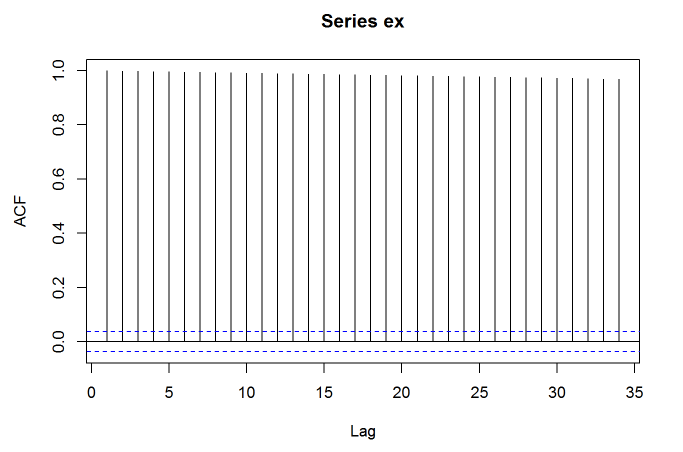
\includegraphics[width=0.6\textwidth]{ex_acf.png} 
\end{center}
\end{figure}
\begin{lstlisting}[language=R] 
origin=da$ExchangeRate
ex=origin[1:2766] # 2005-07-21 To 2016-07-21
acf(ex)
pacf(ex)

# ADF Test
adfTest(ex,lags=m1$order,type=c("c"))
## 
## Title:
##  Augmented Dickey-Fuller Test
## 
## Test Results:
##   PARAMETER:
##     Lag Order: 12
##   STATISTIC:
##     Dickey-Fuller: -3.1048
##   P VALUE:
##     0.0274 
\end{lstlisting}

However, when we want to further estimate a ARIMA model, the autocorrelation between the 8th difference exchange rate are still significant at lag 13th. Unlike Zhang(2005) who successfully estimated am $ARIMA(2,4,5)$ model using monthly data from Jan. 1989 to Dec. 2003, our estimation using daily data, an $ARIMA(6,4,12)$ model, failed to adequately estimate the results. Thus, we focus on ARCH and GARCH model in the following research.

\subsection{Autoregressive Conditional Heteroscedastic Model}
The basic idea of Autoregressive Conditional Heteroscedastic(ARCH) model is that ${a_t}$is a serially uncorrelated but dependent, and the dependence of $a_t$ can be described by a simple quadratic function of the lagged value. An $ARCH(m)$ model is like
\begin{eqnarray*}
a_t &=& \sigma_t \epsilon_t \\
\sigma_t^2 &=& \alpha_0 + \alpha_1 a_{t-1}^2 + \cdots +\alpha_m a_{t-m}^2
\end{eqnarray*}

Consider previous researches' experience, we first estimate an ARCH(1) model, results are like
\begin{eqnarray*}
r_t &=& 1.9966 + a_t\\
\sigma_t^2 &=& 6.055*10^{-07} + 1.000 a_{t-1}^2 
\end{eqnarray*}
\begin{figure}[h!]
\begin{center}
\caption{ARCH(1)}\label{ARCH(1)}
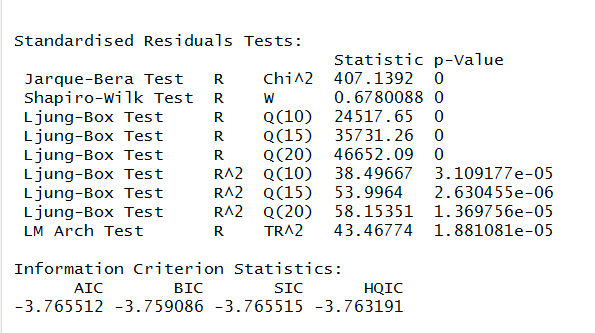
\includegraphics[width=0.6\textwidth]{arch1a.png} 
\end{center}
\end{figure}

And also an ARCH(3) model,
\begin{eqnarray*}
r_t &=& 1.9966 + a_t\\
\sigma_t^2 &=& 5.675*10^{-7} + 0.9953 a_{t-1}^2 + 1.000*10^{-8} a_{t-2}^2 +0.01381 a_{t-3}^2
\end{eqnarray*}
\begin{figure}[h!]
\begin{center}
\caption{ARCH(3)}\label{ARCH(3)}
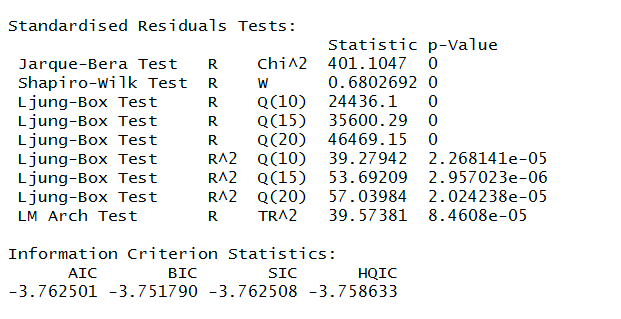
\includegraphics[width=0.6\textwidth]{arch3a.png} 
\end{center}
\end{figure}


\subsection{General Autoregressive Conditional Heteroscedastic Model}
A General Autoregressive Conditional Heteroscedastic(GARCH) model is an extension of Autoregressive Conditional Heteroscedastic(ARCH) model. It shows the parsimonious of the parameters to adequately describe the volatility process of a series. The most commonly used GARCH model is $GARCH(1,1)$, and its form is like $a_t = \sigma_t \epsilon_t$, $\sigma^2 = \alpha_0 + \alpha_1 a_{t-1}^2 + \beta_1 \sigma_{t-1}^2$ where $0 \leq \alpha_1, \beta_1 \leq 1, (\alpha_1 + \beta_1) <1$.\\ 

Thus we estimate an GARCH(1,1) model,
\begin{eqnarray*}
r_t &=& 2.0576 + a_t\\
\sigma_t^2 &=& 6.144*10^{-9} + 0.1619 a_{t-1}^2 + 0.8440 \sigma_{t-3}^2
\end{eqnarray*}
\begin{figure}[h!]
\begin{center}
\caption{GARCH(1,1)}\label{GARCH(1,1)}
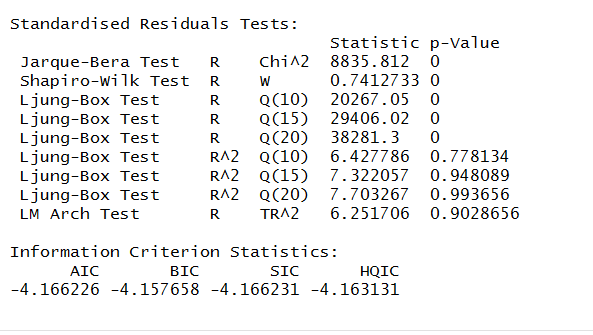
\includegraphics[width=0.6\textwidth]{garch11a.png} 
\end{center}
\end{figure}

\section{Estimation and Result Analysis}
As the results above, we can find the $GARCH(1,1)$ model have the highest likelihood with the lowest AIC and BIC, while the considering the significance of parameters $\alpha_2$ and $\alpha_3$, $ARCH(1)$ model is more appropriate than the $ARCH(3)$ model. Further, Ljung box test is needed to decide which model is better. Ljung box test can be used to test the validity of the mean equation and the volatility equation by checking the autocorrelation between the standardized residuals. If p value is less than $0.05$, we can reject the null hypothesis, seeing the model is appropriate. As we can see from the results, $GARCH(1,1)$ model is suitable for the volatility and mean equation.\\

The prediction we make using the estimated $GARCH(1,1)$ model is like figure \ref{pre}.
\begin{figure}[h!]
\begin{center}
\caption{point forecast}\label{pre}
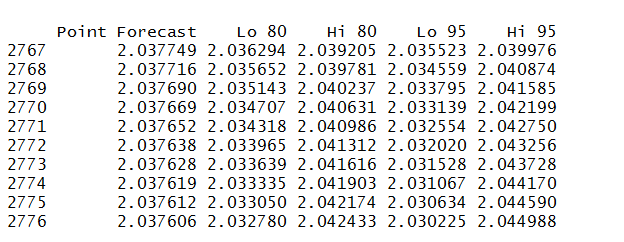
\includegraphics[width=0.6\textwidth]{pre.png}
\end{center}
\end{figure}


\section{Conclusions}
While what really disappoint us is that the forecast is not consistent with the actual value, shown as figure \ref{volatility}. Having seen from the result, the test results showed the detection model did not possesses preferable practicability. The exchange rate volatility shows the forecast result is not consistent with the actual series in GARCH model.\\
\begin{figure}[h!]
\begin{center}
\caption{}\label{volatility}
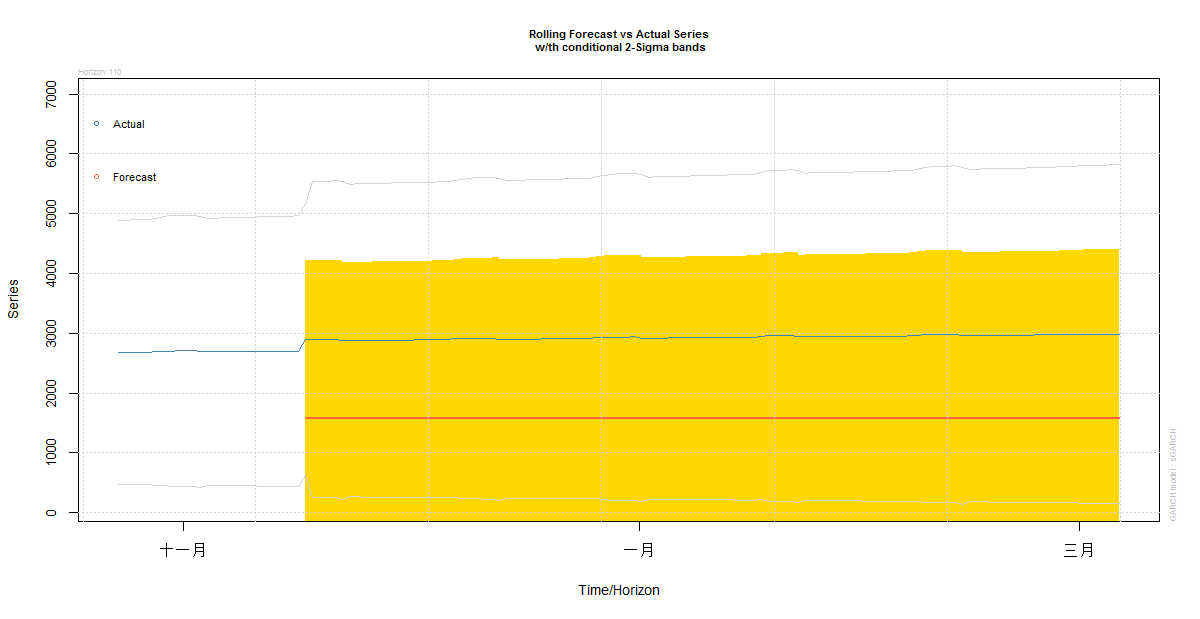
\includegraphics[width=0.6\textwidth]{forecast.jpg}
\end{center}
\end{figure}

This method have error, which might be the factor that make the estimate result is not pretty ideal. Due to time limitation, we are not sure what problem causes this inaccuracy result, which we may try to discuss in the future. According to the analysis, we can see the exchange rate fluctuated remarkably, which is not normal distribution. It seems infeasible to use this model to predict the exchange rate revealing the upward tendency for the CNY. Along with the Special Drawing Right(SDR), CNY gradually move in the line with the trend of the international financial market, while the non-stationary means it still needs to take measures to prevent the risk of the sharp appreciation and depreciation.\\

\begin{thebibliography}{9}
\bibitem{}  Fang-Mei Tseng,Gwo-Hshiung Tzeng,Hsiao-Cheng Yu,Benjamin J. C. Yuan. Fuzzy ARIMA model for forecasting the foreign exchange market.[J]. Fuzzy Sets and Systems,2001,118:.
\bibitem{}  Federal Reserve System. https://www.federalreserve.gov/datadownload/Choose.aspx?rel=H10 
\bibitem{}  Hui X F, Xing L. Analysis of the RMB exchange rate formation mechanism based on the currency basket[C]. International Conference on Management Science \& Engineering. IEEE, 2014:1101-1105. 
\bibitem{}  Liu S L, Wen T, Jun G E. Forecasting and the Choice of RMB Exchange Rate Model——Base on ARIMA Model and GARCH Model[J]. Technoeconomics \& Management Research, 2008.
\bibitem{}  Luo X. The Research of the Fluctuation Rules of USD/RMB Exchange Rate Series Based on GARCH Model[J]. Application of Statistics \& Management, 2009, 28(2):295-300.
\bibitem{}  Marco Mele. A “TIME SERIES” APPROACH ON THE CHINESE EXCHANGE RATE REGIME[J]. Economic Research,2010,233:.
\bibitem{}  O'Sullivan, Arthur; Steven M. Sheffrin (2003). Economics: Principles in action. Upper Saddle River, New Jersey 07458: Pearson Prentice Hall. p. 458.ISBN 0-13-063085-3. 
\bibitem{}  Tsay, Ruey S. Analysis of Financial Time Series. Analysis of financial time series. Wiley, 2005:5880-5885.
\bibitem{}  Wu M Q, The study on the fluctuation trend of US dollar to RMB exchange rate -- Based on GARCH model [J]. Journal of Tongling University. 2016,06:27-30+55.
\bibitem{}  Xu S Q, Li Y M.Prediction of RMB exchange rate with reference to a basket of currencies -- an empirical method based on ARMA model. [J]. World Economic Papers. 2007(03)
\bibitem{}  Yang S F. Time series modeling and prediction [D]. Tsinghua University. 2014.
\bibitem{}  Zhai A M. The Empirical Research of RMB Exchange Rate Volatility Based on GARCH Model[J]. Technoeconomics \& Management Research, 2010.
\end{thebibliography}


\section*{Appendix}
\subsection*{Additional R code}
\begin{lstlisting}[language=R] 
library(readxl)
library(timeDate)
library(timeSeries)
library(TSA)
library(fUnitRoots)
library(forecast)

data <- read_excel("D:/Junior/GitHub/FDA_project_LYF/Data/MonthlyData.xls")

head(data)
dim(data)

plot(data,type="l")

da <- read_excel("D:/Junior/GitHub/FDA_project_LYF/Data/DailyData.xlsx")

head(da)
dim(da)

plot(da,type="l")

# Take difference
dex2=diff(dex)
dex3=diff(dex2)
dex4=diff(dex3)
dex5=diff(dex4)
dex6=diff(dex5)
dex7=diff(dex6)
dex8=diff(dex7)
acf(dex8)
pacf(dex8)

#ARIMA
m2=arima(ex,c(6,4,12))
m2
Box.test(m2$residuals,lag=30,type = "Ljung")
pv2=1-pchisq(776.93,12)
pv2


Call:
arima(x = ex, order = c(6, 4, 12))

Coefficients:
          ar1      ar2     ar3      ar4     ar5      ar6      ma1     ma2
      -0.8638  -0.1001  0.0419  -0.0185  0.0187  -0.0084  -1.6103  0.3084
s.e.      NaN      NaN     NaN      NaN     NaN   0.0004      NaN  0.0003
         ma3      ma4     ma5     ma6     ma7      ma8     ma9    ma10     ma11
      0.2579  -0.0777  0.1486  -0.033  0.0986  -0.0976  0.1079  -0.095  -0.1169
s.e.     NaN      NaN  0.0001     NaN  0.0002      NaN     NaN     NaN   0.0004
        ma12
      0.1103
s.e.  0.0003

sigma^2 estimated as 0.0001398:  log likelihood = 8328.14,  aic = -16620.28

	Box-Ljung test

data:  m2$residuals
X-squared = 776.93, df = 30, p-value < 2.2e-16
\end{lstlisting}
\end{document}
